\chapter{Image 1}
\label{chap:image1}

\begin{figure}[!ht]
	\begin{subfigure}{.49\textwidth}
		\centering
		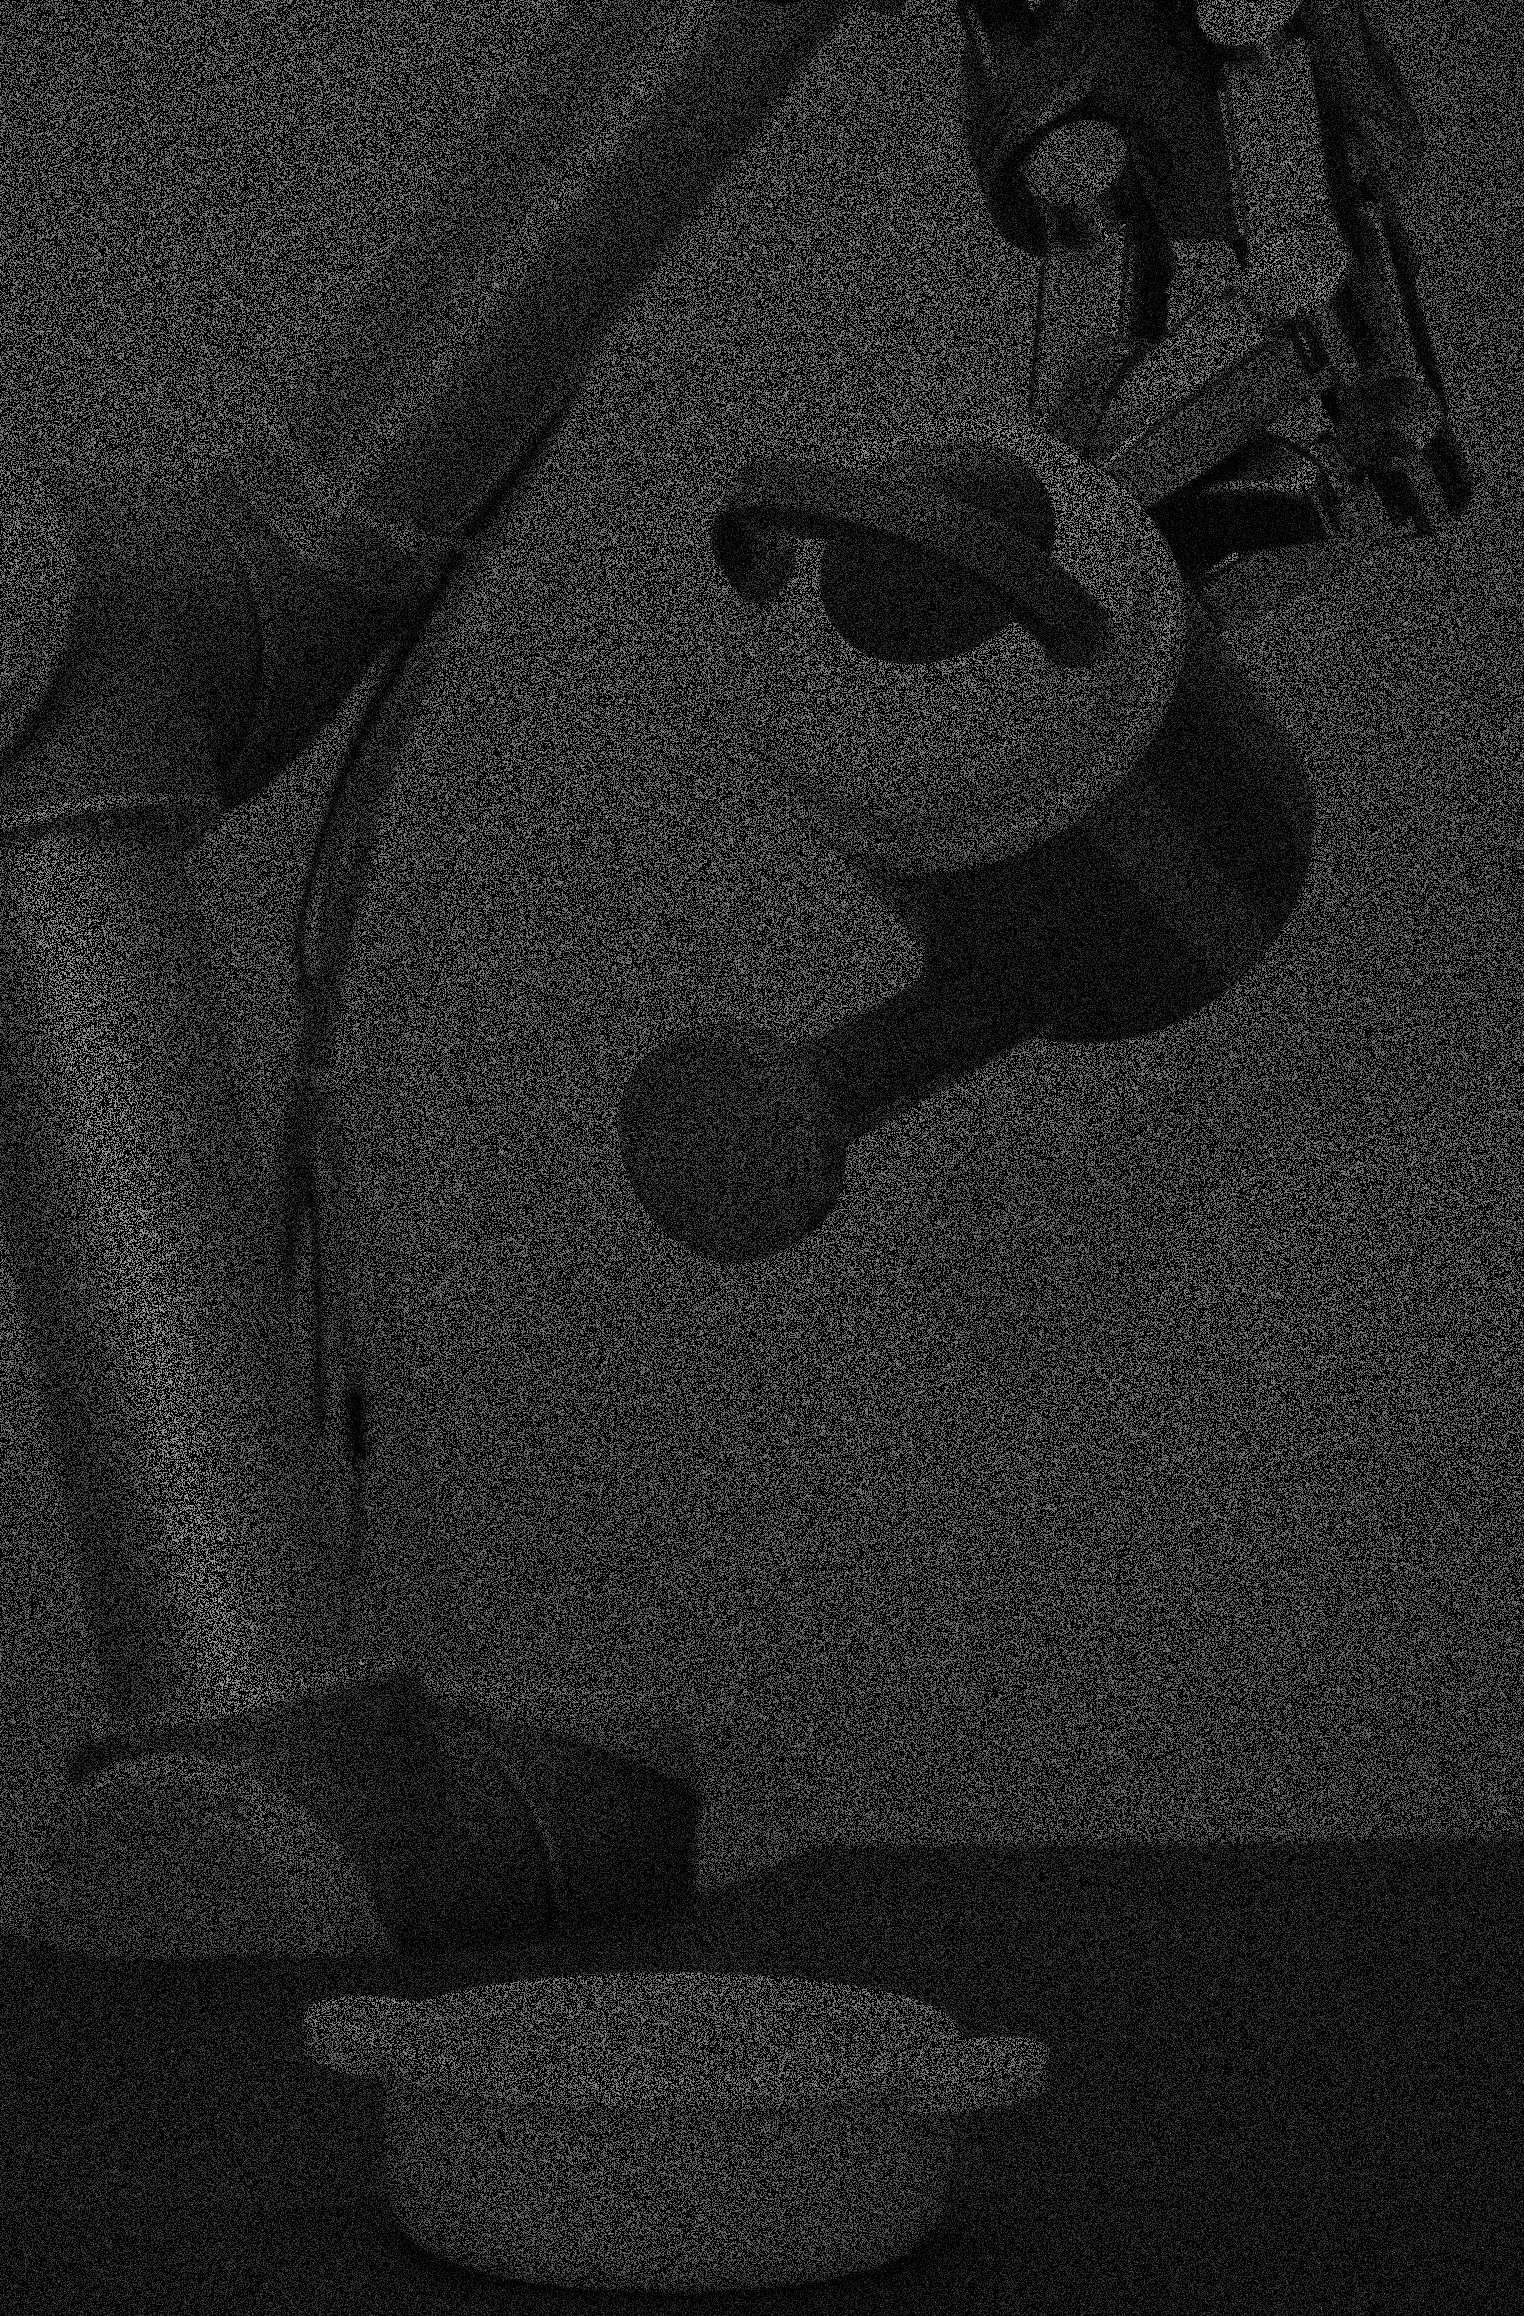
\includegraphics[width=1\textwidth]{figures/1-imageOriginal}
		\caption{Original image}
		\label{fig:1-ImageOriginalSmall}
	\end{subfigure}
	\begin{subfigure}{.49\textwidth}
		\centering
		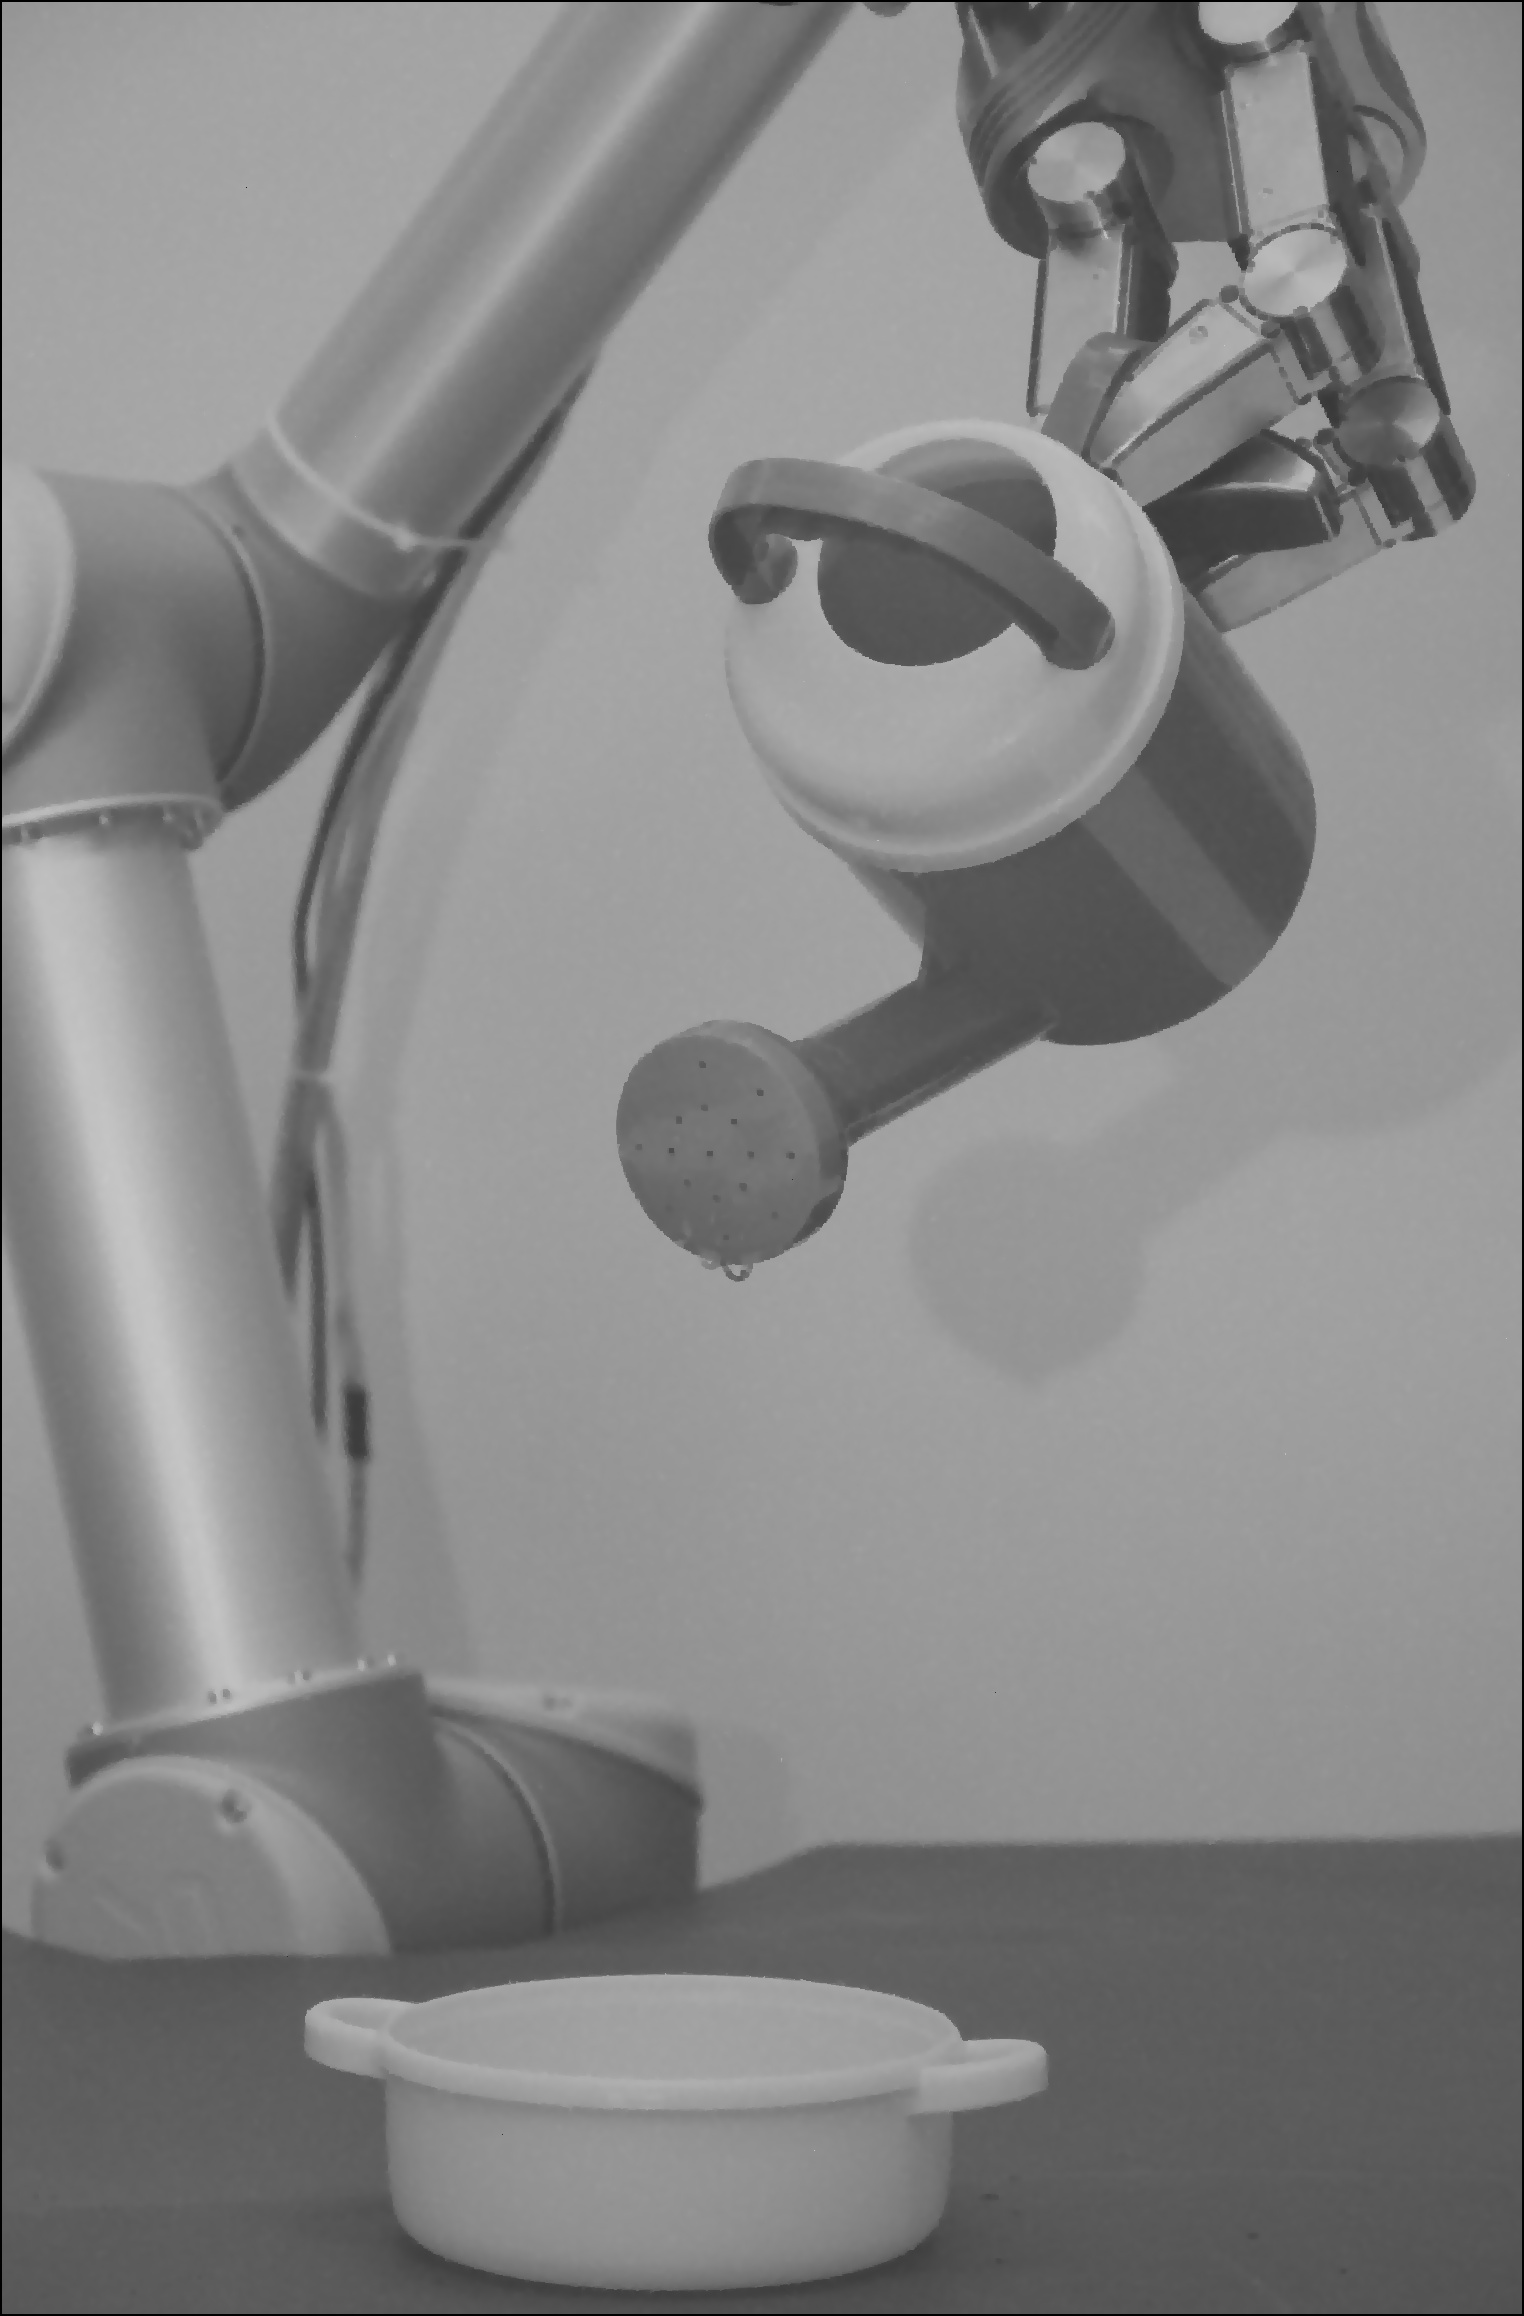
\includegraphics[width=1\textwidth]{figures/1-imageFiltered}
		\caption{Restored image}
		\label{fig:1-ImageFilteredSmall}
	\end{subfigure}
\caption{Original and restored images.}
\label{fig:1-originalAndRestored}
\end{figure}

In the figure \ref{fig:1-originalAndRestored} the image 1 and its final result is presented. The original image shows a big quantity of black pixels (pepper) and in the following sections is explained the process to detect and resolve that problem.

\section{Procedure}
\label{sec:image1_procedure}
The original image (figure \ref{fig:1-ImageOriginalSmall}), presents a big quantity of black pixels that should be fixed. This problem can be observed better in the figure \ref{fig:1-noiseDetail} where a big part of the pixels is black.

\begin{figure}[!ht]
	\centering
	
\includegraphics[width=0.5\textwidth]{figures/1-noiseDetail}
	\caption{Noise detail in image 1.}
	\label{fig:1-noiseDetail}
\end{figure}

In the histogram analysis, showed in figure \ref{fig:1-histogramOriginal}, the most of the accumulation is presented in the black region so the idea of an excess of black pixels is reinforced.

\begin{figure}[!ht]
	\centering
	
\includegraphics[width=0.8\textwidth]{figures/1-histogramOriginal}
	\caption{Single-channel histogram from the original image 1.}
	\label{fig:1-histogramOriginal}
\end{figure}

To solve this kind of problems we can apply different solutions, as the order-statistics filters. Inside of this family filters one of the best known for solve this problem is a filter of maximum. Another solution is based in the same idea of the kernel but, in spite of take the maximum, take an intermediate value, as the median. 

It consists in that for each pixel, the surrounded pixels are analyze and sorted so the pixel with the maximum value is put in the first pixel. This means that if you are working in a black pixel and you take the 8 surrounded pixels, the value will be change for the whitest founded if you decide to make a maximum filter, or another whiter pixel depending on you decision.

There are many parameters to modify in this filter as for example the number of pixels you analyze or in which direction is done.

After different experiments we finally get our optimal configuration being this a filter a slightly different filter from the median filter but based on the same idea. What the filter does is divided in to parts, as shown in figure \ref{fig:1-filterCode}.

\begin{figure}[!ht]
	\centering
	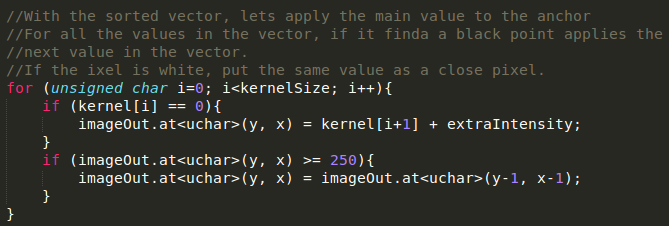
\includegraphics[width=0.95\textwidth]{figures/1-filterCode}
	\caption{Code implementation of the pixel decision in the image 1's filter.}
	\label{fig:1-filterCode}
\end{figure}

On the one hand, for all the black points, the next to this is stored in the pixel filtered. This means that the immediately next value to a black pixel is the chosen. On the other hand, if this value is whiter, is discarded, and the value of a close pixel is taken. Also, in this part, a extra intensity can be added so intensity adjustments can be made.

Finally a bilateral filter is applied to the output image. The bilateral filter \cite{bilateralFilter} normalize the colors respecting the borders, so the small color differences between close pixels is removed and the output image seems to be more regular as in the original image.

\section{Observations and Data}
\label{sec:image1_observations}

\begin{figure}[!ht]
	\centering
	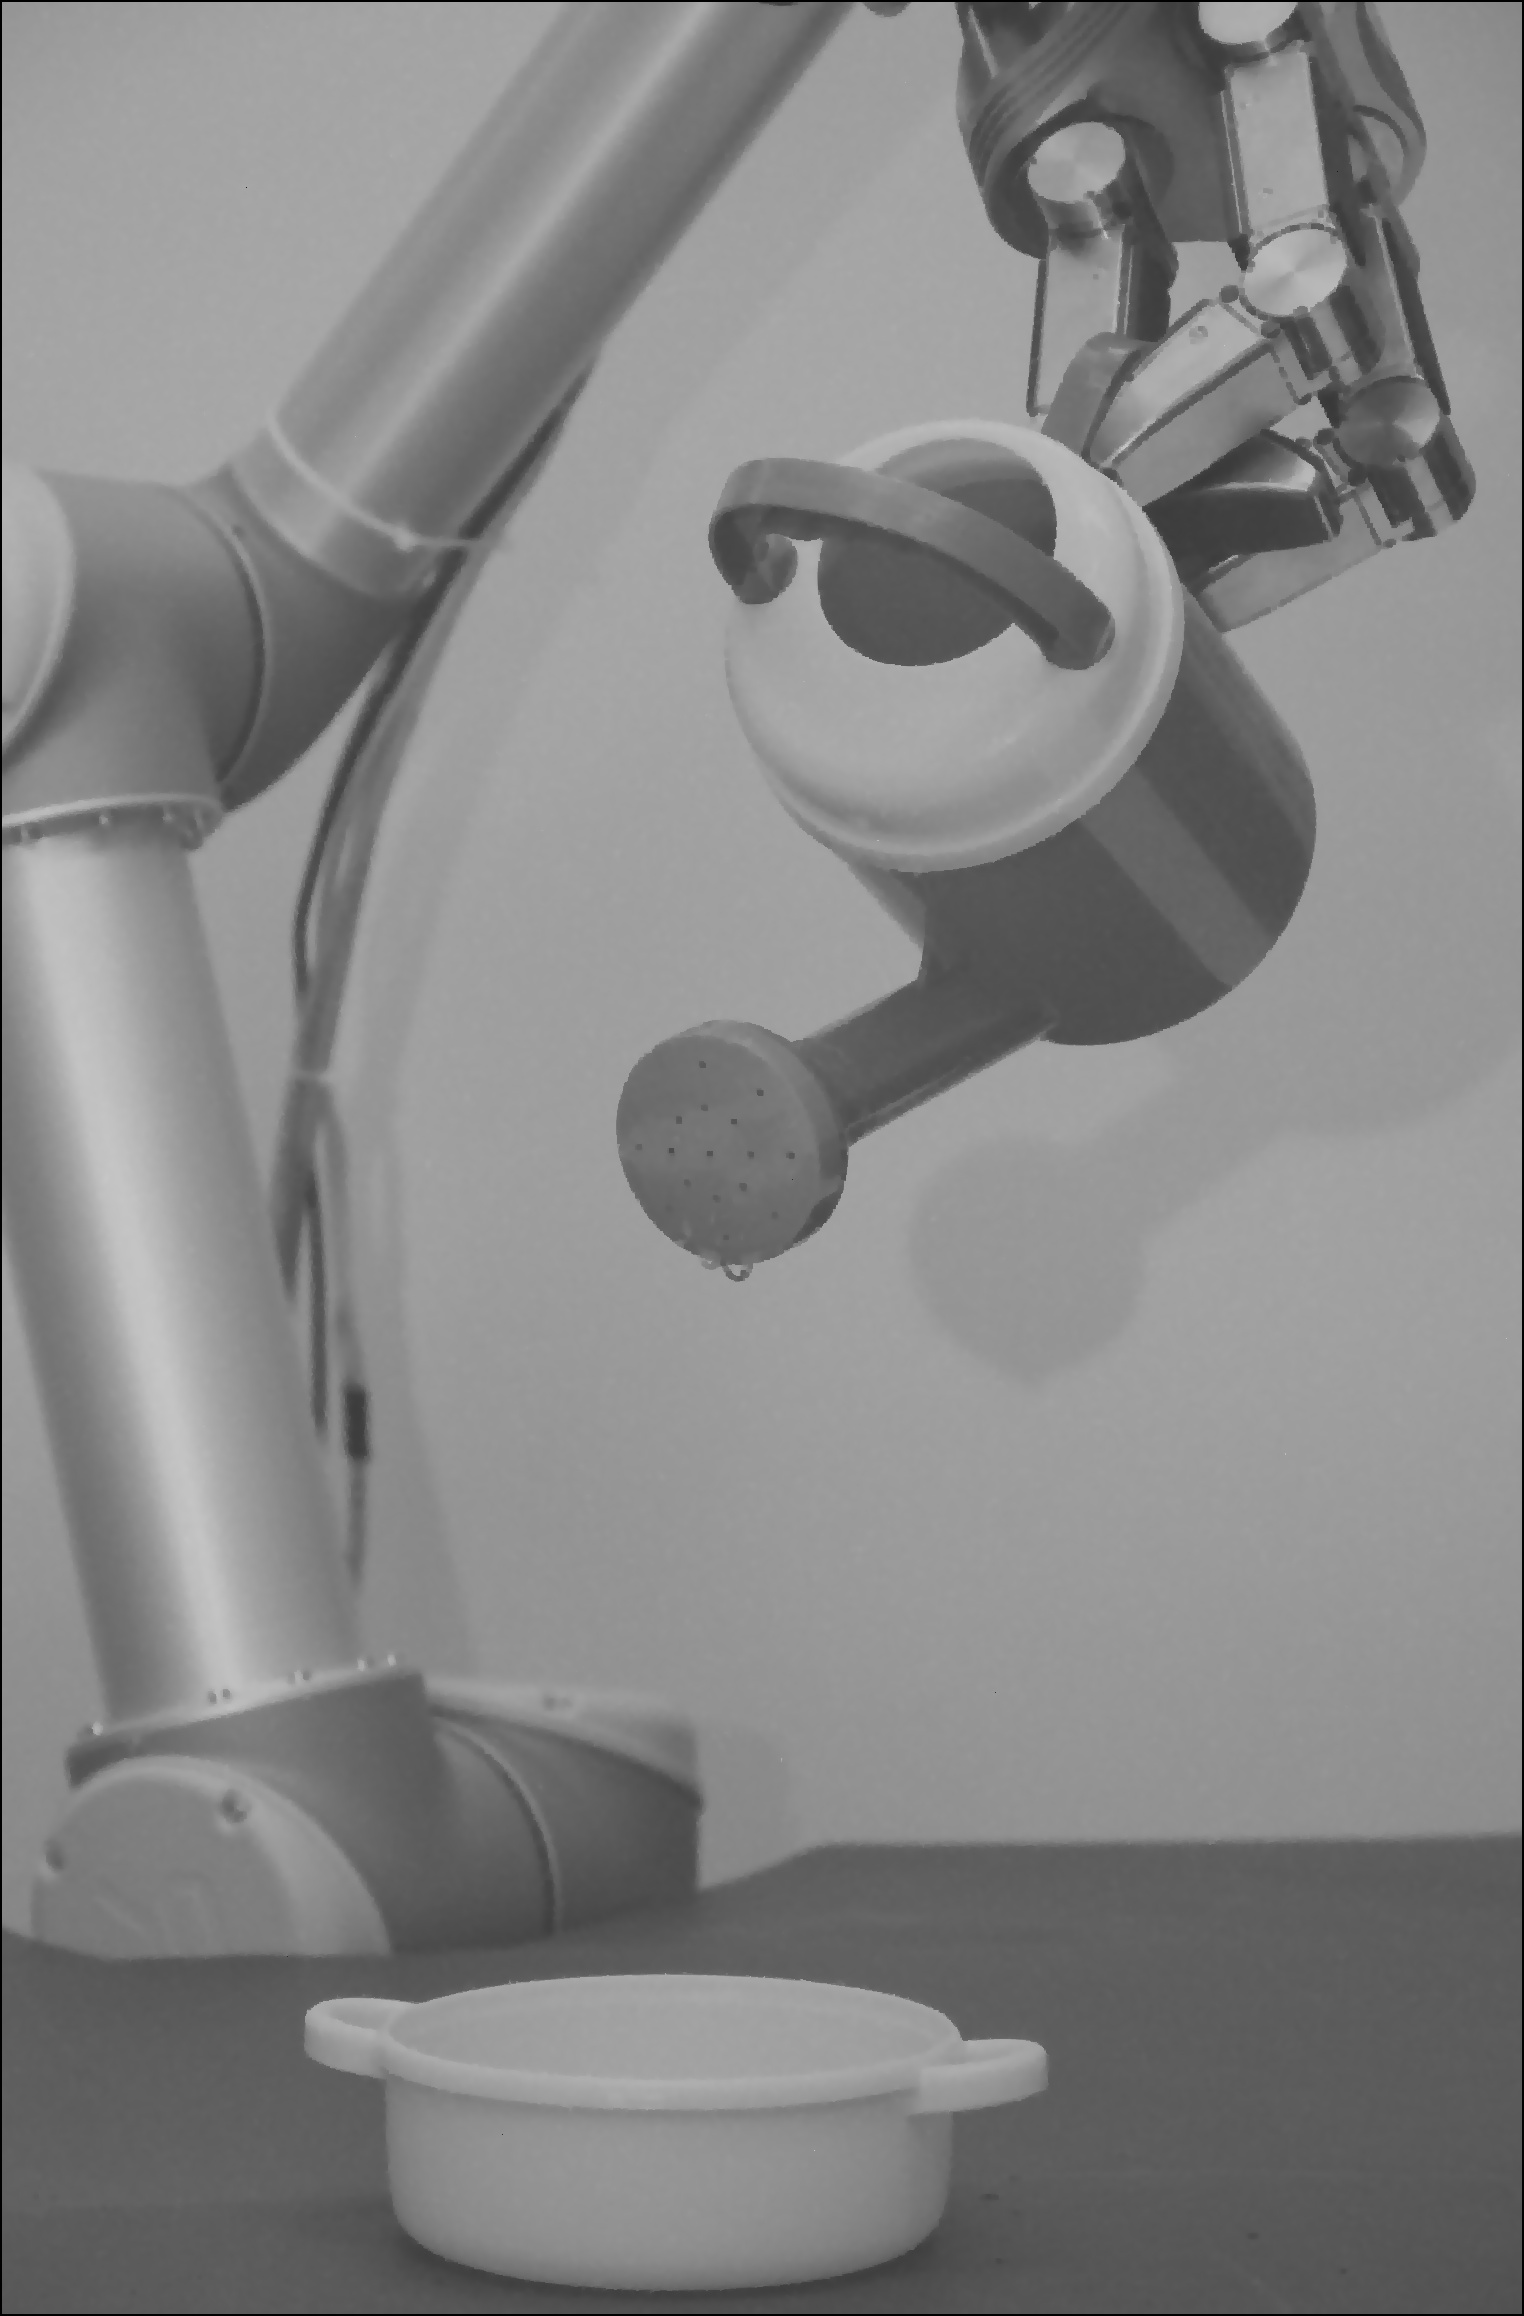
\includegraphics[height=0.75\textheight]{figures/1-imageFiltered}
	\caption{Final filtered image 1.}
	\label{fig:1-imageFiltered}
\end{figure}

The output image is shown bigger in the figure \ref{fig:1-imageFiltered} and a detail of the same area as before is presented in figure \ref{fig:1-filteredDetail}.

\begin{figure}[!ht]
	\centering
	
\includegraphics[width=0.5\textwidth]{figures/1-filteredDetail}
	\caption{Pixels detail in the same area as the noise in image 1.}
	\label{fig:1-filteredDetail}
\end{figure}

As it can see from the filtered image detail above, the homogenization is reached thanks to the bilateral filter. On the other hand, the restoration is almost complete having a few problems that are presented now.

The first problem is related with the intensity of the output image. As explained in \ref{sec:image1_procedure}, the immediately to a black pixel is put as the new value, this means that the output image is going to be darker than expected. This problem however, is solved adding an extra intensity being the final histogram as showed in figure \ref{fig:1-histogramFiltered}.

\begin{figure}[!ht]
	\centering
	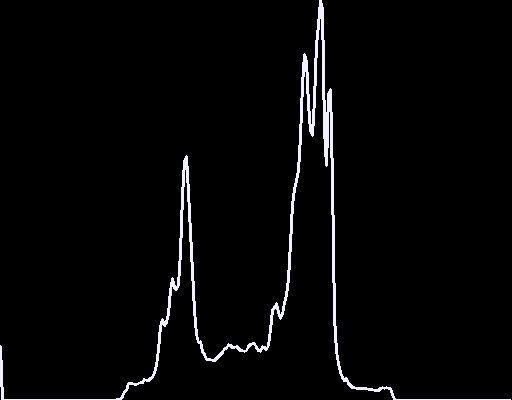
\includegraphics[width=0.8\textwidth]{figures/1-histogramFiltered}
	\caption{Single-channel histogram from the filtered image 1.}
	\label{fig:1-histogramFiltered}
\end{figure}

The second problem is the disappearance of some details along with the blur of the borders. Details as the water can's holes are blured or, actually, removed and all the details are also decreased in part for the big kernel size (25 pixels) and in part for the bilateral filtered that makes disappear the robotic hand's metal glitters for example. 

\section{Analysis of Data}
\label{sec:image1_analysis}
The results achieved are reasonable good comparing the original and the final image. Although is true that details are blured a, more than acceptable result, is reached so we conclude this image. Problems were founded when choosing the filter's kernel size due to the fact to find a balance between computation time, general blurred and homogenization. Despite we test with different kernel size as trying to filter more than once, the best result achieved was found with just one 25 kernel filter and then a bilateral filter.

\section{Conclusions}
\label{sec:image1_conclusions}
Respecting the things we have learn, we have been able to determine the kind of noise we had and also find different ways to attack the noise along with implement them. Respecting ways to improve the image, we think a better result could be found if a sharpener or increaser detail would be implemented in the output, but as the final results were more than acceptable we leave this as future improvements. Also an deeper analysis from the output histogram could be made but this was not carried out due to we don't have the original image's histogram.